\chapter{Calculus review. Plain vanilla options.}

\section{Brief review of differentiation}
The function $ f : \mathbb{R} \rightarrow \mathbb{R} $ is differentiable at the
    point $ x \in \mathbb{R} $ if the limit
\begin{equation*}
    \lim_{h \rightarrow 0} \frac{f(x + h) - f(x)}{h}
\end{equation*}
exists, in which case the derivative $ f'(x) $ is defined as
\begin{equation}
    f'(x) = \lim_{h \rightarrow 0} \frac{f(x + h) - f(x)}{h}.
    \label{eq:definition:derivative}
\end{equation}
\begin{theorem}[Product Rule.]
    The product $ f(x) g(x) $ of two differentiable functions $ f(x) $ and
        $ g(x) $ is differentiable, and
    \begin{equation}
        (f(x) g(x))' = f'(x) g(x) + f(x) g'(x).
        \label{eq:theorem:product-rule}
    \end{equation}
\end{theorem}
\begin{theorem}[Quotient Rule.]
    The quotient $ \frac{f(x)}{g(x)} $ of two differentiable functions $ f(x) $
        and $ g(x) $ is differentiable at every point $ x $ where the function
        $ \frac{f(x)}{g(x)} $ is well defined, and
    \begin{equation}
        \left( \frac{f(x)}{g(x)} \right)' =
            \frac{f'(x) g(x) - f(x) g'(x)}{(g(x))^2}.
        \label{eq:definition:quotient-rule}
    \end{equation}
\end{theorem}
\begin{theorem}[Chain Rule.]
    The composite function $ (g \circ f)(x) = g(f(x)) $ of two differentiable
        functions $ f(x) $ and $ g(x) $ is differentiable at every point $ x $
        where $ g(f(x)) $ is well defined, and
    \begin{equation}
        (g(f(x)))' = g'(f(x)) f'(x).
        \label{eq:definition:chain-rule}
    \end{equation}
\end{theorem}
The Chain Rule formula \eqref{eq:definition:chain-rule} can also be written as
\begin{equation*}
    \frac{dg}{dx} = \frac{dg}{du} \frac{du}{dx},
\end{equation*}
where $ u = f(x) $ is a function of $ x $ and $ g = g(u) = g(f(x)) $.

Chain Rule is often used for power functions, exponential functions, and
    logarithmic function:
\begin{align}
    \frac{d}{dx} ((f(x))^n) &= n (f(x))^{n - 1} f'(x);
        \label{eq:formula:chain-rule:power} \\
    \frac{d}{dx} (e^{f(x)}) &= e^{f(x)} f'(x);
        \label{eq:formula:chain-rule:exp} \\
    \frac{d}{dx} (\ln f(x)) &= \frac{f'(x)}{f(x)}.
        \label{eq:formula:chain-rule:log}
\end{align}

\begin{lemma}
    Let $ f : [a, b] \rightarrow [c, d] $ be a differentiable function, and
        assume that $ f(x) $ has an inverse function denoted by $ f^{-1}(x) $
        with $ f^{-1} : [c, d] \rightarrow [a, b] $.
    The function $ f^{-1}(x) $ is differentiable at every point $ x \in [c, d] $
        where $ f'(f^{-1}(x)) \neq 0 $ and
    \begin{equation}
        (f^{-1}(x))' = \frac{1}{f'(f^{-1}(x))}.
        \label{eq:lemma:inverse}
    \end{equation}
\end{lemma}

\section{Brief review of integration}
Let $ f : \mathbb{R} \rightarrow \mathbb{R} $ be an integrable function.
Recall that $ F(x) $ is the antiderivative of $ f(x) $ iff $ F'(x) = f $, i.e.,
\begin{equation*}
    F(x) = \int f(x) dx \quad \Longleftrightarrow \quad F'(x) = f(x).
\end{equation*}
\begin{theorem}[Fundamental Theorem of Calculus.]
    Let $ f(x) $ be a continuous function on the interval $ [a, b] $, and let
        $ F(x) $ be the antiderivative of $ f(x) $.
    Then
    \begin{equation*}
        \int_{a}^{b} f(x) dx = F(x) |_a^b = F(b) - F(a).
    \end{equation*}
\end{theorem}
Integration by parts is the counterpart for integration of the product rule.
\begin{theorem}[Integration by parts.]
    Let $ f(x) $ and $ g(x) $ be continuous function.
    Then
    \begin{equation}
        \int f(x) g(x) dx = F(x) g(x) - \int F(x) g'(x) dx,
        \label{eq:theorem:int-by-parts}
    \end{equation}
    where $ F(x) = \int f(x) dx $ is the antiderivative of $ f(x) $.
    For definite integrals,
    \begin{equation}
        \int_{a}^{b} f(x) g(x) dx = F(b) g(b) - F(a) g(a) -
            \int_{a}^{b} F(x) g'(x) dx.
        \label{eq:theorem:int-by-parts-definite}
    \end{equation}
\end{theorem}
Integration by substitution if the counterpart for integration of the chain
    rule.
\begin{theorem}[Integration by substitution]
    Let $ f(x) $ be an integrable function.
    Assume that $ g(u) $ is an invertible and continuously differentiable
        function.
    The substitution $ x = g(u) $ changes the integration variable from $ x $
        to $ u $ as follows:
    \begin{equation}
        \int f(x) dx = \int f(g(u)) g'(u) du.
        \label{eq:theorem:int-by-sub}
    \end{equation}
    For definite integrals,
    \begin{equation}
        \int_{a}^{b} f(x) dx = \int_{g^{-1}(a)}^{g^{-1}(b)} f(g(u)) g'(u) du.
        \label{eq:theorem:int-by-sub-definite}
    \end{equation}
\end{theorem}

\section{Differentiating definite integrals}
If a definite integral has functions as limits of integration, e.g.,
\begin{equation*}
    \int_{a(t)}^{b(t)} f(x) dx,
\end{equation*}
or if the function to be integrated is a function of the integrating variable
    and of another variable, e.g.,
\begin{equation*}
    \int_{a}^{b} f(x, t) dx
\end{equation*}
then the result of the integration is a function (of the variable $ t $ in both
    cases above).

\begin{lemma}\label{lemma:int-function-limit}
    Let $ f : \mathbb{R} \rightarrow \mathbb{R} $ be a continuous function.
    Then,
    \begin{equation}
        \frac{d}{dt} \left( \int_{a(t)}^{b(t)} f(x) dx \right) = f(b(t)) b'(t) -
            f(a(t)) a'(t),
        \label{eq:lemma:int-function-limit}
    \end{equation}
    where $ a(t) $ and $ b(t) $ are differentiable functions.
\end{lemma}

\begin{lemma}\label{lemma:int-function-another-var}
    Let $ f : \mathbb{R} \times \mathbb{R} \rightarrow \mathbb{R} $ be a
        continuous function such that the partial derivative
        $ \frac{\partial f}{\partial t} (x, t) $ exists and is continuous in
        both variables $ x $ and $ t $.
    \begin{equation}
        \frac{d}{dt} \left( \int_{a}^{b} f(x, t) dx \right) = \int_{a}^{b}
            \frac{\partial f}{\partial t} (x, t) dx.
        \label{eq:lemma:int-function-another-var}
    \end{equation}
\end{lemma}

\begin{lemma}\label{lemma:int-function-general}
    Let $ f(x, t) $ be a continuous function such that the partial derivative
        $ \frac{\partial f}{\partial t} (x, t) $ exists and is continuous.
    Then,
    \begin{equation*}
        \frac{d}{dt} \left( \int_{a(t)}^{b(t)} f(x, t) dx \right) =
            \int_{a(t)}^{b(t)} \frac{\partial f}{\partial t} (x, t) +
            f(b(t), t) b'(t) - f(a(t), t) a'(t).
    \end{equation*}
\end{lemma}
Note that Lemma \ref{lemma:int-function-limit} and Lemma
    \ref{lemma:int-function-another-var} are special cases of Lemma
    \ref{lemma:int-function-general}.

\section{Limits}
\begin{definition}
    Let $ g : \mathbb{R} \rightarrow \mathbb{R} $.
    The limit of $ g(x) $ as $ x \rightarrow x_0 $ exists and is finite and
        equal to $ l $ iff for any $ \epsilon > 0 $ there exists $ \delta > 0 $
        such that $ |g(x) - l| < \epsilon $ for all $ x \in (x_0 - \delta, x_0 +
        \delta) $, i.e.,
    \begin{equation*}
        \lim_{x \rightarrow x_0} g(x) = l, \quad \text{iff} \quad
            \forall \epsilon > 0 \exists \delta > 0 \quad \text{such that} \quad
            |g(x) - l| < \epsilon,\ \forall |x - x_0| < \delta.
    \end{equation*}
    Similarly,
    \begin{equation*}
        \lim_{x \rightarrow x_0} g(x) = \infty, \quad \text{iff} \quad
            \forall C > 0 \exists \delta > 0 \quad \text{such that} \quad
            g(x) > C,\ \forall |x - x_0| < \delta.
    \end{equation*}
    \begin{equation*}
        \lim_{x \rightarrow x_0} g(x) = -\infty, \quad \text{iff} \quad
            \forall C < 0 \exists \delta > 0 \quad \text{such that} \quad
            g(x) < C,\ \forall |x - x_0| < \delta.
    \end{equation*}
\end{definition}

\begin{theorem}
    If $ P(x) $ and $ Q(x) $ are polynomials and $ c > 1 $ is a fixed constant,
        then
    \begin{align}
        \lim_{x \rightarrow \infty} \frac{P(x)}{c^x} &= 0, \quad
            \forall c > 1; \\
        \lim_{x \rightarrow \infty} \frac{\ln |Q(x)|}{P(x)} &= 0.
    \end{align}
\end{theorem}

\begin{lemma}
    Let $ c > 0 $ be a positive constant.
    Then,
    \begin{align}
        \lim_{x \rightarrow \infty} x^{\frac{1}{x}} &= 1; \\
        \lim_{x \rightarrow \infty} c^{\frac{1}{x}} &= 1; \\
        \lim_{x \searrow 0} x^x &= 1, \\
    \end{align}
    where the notation $ x \searrow 0 $ means that $ x $ goes to 0 while always
        being positive, i.e., $ x \rightarrow 0 $ with $ x > 0 $.
\end{lemma}

\begin{lemma}
    If $ k $ is a positive integer number, and if $ c > 0 $ is a positive fixed
        constant, then
    \begin{align}
        \lim_{k \rightarrow \infty} k^{\frac{1}{k}} &= 1; \\
        \lim_{k \rightarrow \infty} c^{\frac{1}{k}} &= 1; \\
        \lim_{k \rightarrow \infty} \frac{c^k}{k!} &= 0, \\
    \end{align}
    where $ k! = 1 \cdot 2 \cdot ... \cdot k $.
\end{lemma}

\section{L'H\^{o}pital's rule and connections to Taylor expansions}
\begin{theorem}[L'H\^{o}pital's Rule]
    Let $ x_0 $ be a real number; allow $ x_0 = \infty $ and $ x_0 = -\infty $
        as well.
    Let $ f(x) $ and $ g(x) $ be two differentiable functions.
    \begin{enumerate}[label=(\roman*)]
        \item Assume that $ \lim_{x \rightarrow x_0} f(x) = 0 $ and
                $ \lim_{x \rightarrow x_0} g(x) = 0 $.
            If $ \lim_{x \rightarrow x_0} \frac{f'(x)}{g'(x)} $ exists, and if
                there exists an interval $ (a, b) $ around $ x_0 $ such that
                $ g'(x) \neq 0 $ for all $ x \in (a, b) \setminus 0 $, then the
                limit $ \lim_{x \rightarrow x_0} \frac{f(x)}{g(x)} $ also exists
                and
            \begin{equation*}
                \lim_{x \rightarrow x_0} \frac{f(x)}{g(x)} =
                    \lim_{x \rightarrow x_0} \frac{f'(x)}{g'(x)}.
            \end{equation*}
        \item Assume that $ \lim_{x \rightarrow x_0} f(x) $ is either
                $ -\infty $ or $ \infty $, and that $ \lim_{x \rightarrow x_0}
                g(x) $ is either $ -\infty $ or $ \infty $.
            If the limit $ \lim_{x \rightarrow x_0} \frac{f'(x)}{g'(x)} $
                exists, and if there exists an interval $ (a, b) $ around
                $ x_0 $ such that $ g'(x) \neq 0 $ for all $ x \in (a, b)
                \setminus 0 $, then the limit $ \lim_{x \rightarrow x_0}
                \frac{f(x)}{g(x)} $ also exists and
            \begin{equation*}
                \lim_{x \rightarrow x_0} \frac{f(x)}{g(x)} =
                    \lim_{x \rightarrow x_0} \frac{f'(x)}{g'(x)}.
            \end{equation*}
    \end{enumerate}
\end{theorem}

\section{Multivariable functions}
\paragraph{Scalar Valued Functions}
Let $ f : \mathbb{R}^n \rightarrow \mathbb{R} $ be a function of $ n $ variables
    denoted by $ x_1, x_2, ..., x_n $, and let $ x = (x_1, x_2, ..., x_n) $.

\begin{definition}
    Let $ f : \mathbb{R}^n \rightarrow \mathbb{R} $.
    The partial derivative of the function $ f(x) $ with respect to the variable
        $ x_i $ is denoted by $ \frac{\partial f}{\partial x_i} (x) $ and is
        defined as
    \begin{equation}
        \frac{\partial f}{\partial x_i} (x) = \lim_{h \rightarrow 0}
            \frac{f(x_1, ..., x_{i - 1}, x_i + h, x_{i + 1}, ..., x_n) -
            f(x_1, x_2, ..., x_n)}{h},
        \label{eq:definition:partial-derivative-scalar-valued-function}
    \end{equation}
    if the limit from \eqref{eq:definition:partial-derivative-scalar-valued-function}
        exists and is finite.
\end{definition}

A compact formula for \eqref{eq:definition:partial-derivative-scalar-valued-function}
    can be given as follows:
Let $ e_i $ be the vector with all entries equal to 0 with the exception of the
    i-th entry, which is equal for 1, i.e., $ e_i(j) = 0 $, for $ j \neq i $,
    $ 1 \leq j \leq n $, and $ e_i(j) = 1 $. Then,
\begin{equation*}
    \frac{\partial f}{\partial x_i}(x) = \lim_{h \rightarrow 0}
        \frac{f(x + h e_i) - f(x)}{h}.
\end{equation*}

\begin{theorem}
    If all the partial derivatives of order $ k $ of the function $ f(x) $ exist
        and are continuous, then the order in which partial derivatives of
        $ f(x) $ of order at most $ k $ is computed does not matter.
\end{theorem}

\begin{definition}
    Let $ f : \mathbb{R}^n \rightarrow \mathbb{R} $ be a function of $ n $
        variables and assume that $ f(x) $ is differentiable with respect to all
        variables $ x_i $, $ i = 1 : n $.
    The gradient $ D f(x) $ of the function $ f(x) $ is the following row vector
        of size $ n $:
    \begin{equation}
        D f(x) = \left( \frac{\partial f}{\partial x_1} (x)
            \frac{\partial f}{\partial x_2} (x) \cdots
            \frac{\partial f}{\partial x_n} (x) \right).
        \label{eq:definition:partial-derivative-scalar-valued-function-gradient}
    \end{equation}
\end{definition}

\begin{definition}
    Let $ f : \mathbb{R}^n \rightarrow \mathbb{R} $ be a function of $ n $
        variables.
    The Hessian of $ f(x) $ is denoted by $ D^2 f(x) $ and is defined as the
        following $ n \times n $ matrix:
    \begin{equation}
        D^2 f(x) =
        \begin{pmatrix}
            \frac{\partial^2 f}{\partial x_1^2} (x) &
                \frac{\partial^2 f}{\partial x_2 \partial x_1} (x) & \cdots &
                \frac{\partial^2 f}{\partial x_n \partial x_1} (x) \\
            \frac{\partial^2 f}{\partial x_1 \partial x_2} (x) &
                \frac{\partial^2 f}{\partial x_2^2} (x) & \cdots &
                \frac{\partial^2 f}{\partial x_n \partial x_2} (x) \\
            \vdots & \vdots & \ddots & \vdots \\
            \frac{\partial^2 f}{\partial x_1 \partial x_n} (x) &
                \frac{\partial^2 f}{\partial x_2 \partial x_n} (x) & \cdots &
                \frac{\partial^2 f}{\partial x_n^2} (x)
        \end{pmatrix}.
        \label{eq:definition:partial-derivative-scalar-valued-function-hessian}
    \end{equation}
\end{definition}
Another commonly used notations for the gradient and Hessian of $ f(x) $ are
    $ \nabla f(x) $ and $ H f(x) $, respectively.

\paragraph{Vector Valued Functions}
Let $ F : \mathbb{R}^n \rightarrow \mathbb{R}^m $ be a vector valued function
    given by
\begin{equation*}
    F(x) =
    \begin{pmatrix}
        f_1 (x) \\
        f_2 (x) \\
        \vdots \\
        f_m (x)
    \end{pmatrix},
\end{equation*}
where $ x = (x_1, x_2, ..., x_n) $.

\begin{definition}
    Let $ F : \mathbb{R}^n \rightarrow \mathbb{R}^m $ given by
        $ F(x) = (f_j(x))_{j=1:m)} $, and assume that the functions $ f_j(x) $,
        $ j = 1:m $, are differentiable with respect to all variables
        $ x_i = 1:n $.
    The gradient $ D F(x) $ of the function $ F(x) $ is the following matrix of
        size $ m \times n $:
    \begin{equation}
        D F(x) =
        \begin{pmatrix}
            \frac{\partial f_1}{\partial x_1} (x) &
                \frac{\partial f_1}{\partial x_2} (x) & \cdots &
                \frac{\partial f_1}{\partial x_n} (x) \\
            \frac{\partial f_2}{\partial x_1} (x) &
                \frac{\partial f_2}{\partial x_2} (x) & \cdots &
                \frac{\partial f_2}{\partial x_n} (x) \\
            \vdots & \vdots & \ddots & \vdots \\
            \frac{\partial f_m}{\partial x_1} (x) &
                \frac{\partial f_m}{\partial x_2} (x) & \cdots &
                \frac{\partial f_m}{\partial x_n} (x)
        \end{pmatrix}.
        \label{eq:definition:partial-derivative-vector-valued-function-gradient}
    \end{equation}
\end{definition}

\subsection{Functions of two variables}
\paragraph{Scalar Valued Functions}
Let $ f : \mathbb{R}^2 \rightarrow \mathbb{R} $ be a function of two variables
    denoted by $ x $ and $ y $.
The partial derivatives of the function $ f(x, y) $ with respect to the
    variables $ x $ and $ y $ are denoted by $ \frac{\partial f}{\partial x}
    (x, y) $ and $ \frac{\partial f}{\partial y} (x, y) $, respectively, and
    defined as follows:
\begin{align*}
    \frac{\partial f}{\partial x} (x, y) &= \lim_{h \rightarrow 0}
        \frac{f(x + h, y) - f(x, y)}{h}; \\
    \frac{\partial f}{\partial y} (x, y) &= \lim_{h \rightarrow 0}
        \frac{f(x, y + h) - f(x, y)}{h}.
\end{align*}
The gradient of $ f(x, y) $ is
\begin{equation}
    D f(x, y) =
    \begin{pmatrix}
        \frac{\partial f}{\partial x} (x, y) &
            \frac{\partial f}{\partial y} (x, y)
    \end{pmatrix}.
    \label{eq:definiton:two-variable-scalar-function-gradient}
\end{equation}
The Hessian of $ f(x, y) $ is
\begin{equation}
    D^2 f(x, y) =
    \begin{pmatrix}
        \frac{\partial^2 f}{\partial x^2} (x, y) &
            \frac{\partial^2 f}{\partial y \partial x} (x, y) \\
        \frac{\partial^2 f}{\partial x \partial y} (x, y) &
            \frac{\partial^2 f}{\partial y^2} (x, y)
    \end{pmatrix}.
    \label{eq:definition:two-variable-scalar-function-hessian}
\end{equation}

\paragraph{Vector Valued Functions}
Let $ F : \mathbb{R}^2 \rightarrow \mathbb{R}^2 $ given by
\begin{equation*}
    F(x, y) =
    \begin{pmatrix}
        f_1(x, y) \\
        f_2(x, y)
    \end{pmatrix}.
\end{equation*}
The gradient of $ F(x, y) $ is
\begin{equation}
    D F(x, y) =
    \begin{pmatrix}
        \frac{\partial f_1}{\partial x} (x, y) &
            \frac{\partial f_1}{\partial y} (x, y) \\
        \frac{\partial f_2}{\partial x} (x, y) &
            \frac{\partial f_2}{\partial y} (x, y)
    \end{pmatrix}.
    \label{eq:definition:two-variable-vector-function-gradient}
\end{equation}

\section{Plain vanilla European Call and Put options}
\paragraph{Call Option}
A Call Option on an underlying asset is a contract between two parties which
    gives the buyer of the option the right, but not the obligation, to
    \textbf{buy} from the seller of the option one unit of the asset at a
    predetermined time $ T $ in the future, call the maturity of the option, for
    a predetermined price $ K $, call the strike of the option.
For this right, the buyer of the option pays $ C(t) $ at time $ t < T $ to the
    seller of the option.

\paragraph{Put Option}
A Put Option to an underlying asset is a contract between two parties which
    gives the buyer of the option the right, but not the obligation, to
    \textbf{sell} to the seller of the option one unit of the asset at a
    predetermined time $ T $ in the future, called the maturity of the option,
    for a predetermined price $ K $, called the strike of the option.
For this right, the buyer of the option pays $ P(t) $ at time $ t < T $ to the
    seller of the option.

The options described above are plain European options.
An American option can be exercised at any time prior to maturity.

In an option contract, two parties exist: the buyer of the option and the seller
    of the option.
The buyer of the option is long the option (or has a long position in the
    option) and the seller of the option is short the option (or has a short
    position in the option).

Let $ S(t) $ and $ S(T) $ be the price of the underlying asset at time $ t $ and
    at maturity $ T $, respectively.

At time $ t $, a call option is
\begin{equation*}
    \begin{cases}
        ITM & \text{if} \quad S(t) > K; \\
        ATM & \text{if} \quad S(t) = K; \\
        OTM & \text{if} \quad S(t) < K, \\
    \end{cases}
\end{equation*}
where ITM is in the money, ATM is at the money, and OTM is out of the money
    (OTM).
A put option is
\begin{equation*}
    \begin{cases}
        ITM & \text{if} \quad S(t) < K; \\
        ATM & \text{if} \quad S(t) = K; \\
        OTM & \text{if} \quad S(t) > K.
    \end{cases}
\end{equation*}

At maturity $ T $, a call option expires
\begin{equation*}
    \begin{cases}
        ITM & \text{if} \quad S(T) > K; \\
        ATM & \text{if} \quad S(T) = K; \\
        OTM & \text{if} \quad X(T) < K.
    \end{cases}
\end{equation*}
A put option expires
\begin{equation*}
    \begin{cases}
        ITM & \text{if} \quad S(T) < K; \\
        ATM & \text{if} \quad S(T) = K; \\
        OTM & \text{if} \quad X(T) > K.
    \end{cases}
\end{equation*}

The payoff of a call option at maturity is
\begin{equation*}
    C(T) = \max (S(T) - K, 0) =
    \begin{cases}
        S(T) - K, & \text{if} \quad S(T) > K; \\
        0, & \text{if} \quad S(T) \leq K. \\
    \end{cases}
\end{equation*}
The payoff of a put option at maturity is
\begin{equation*}
    P(T) = \max (K - S(T), 0) =
    \begin{cases}
        0, & \text{if} \quad S(T) \geq K; \\
        K - S(T), & \text{if} \quad S(T) < K. \\
    \end{cases}
\end{equation*}

\section{Arbitrage-free pricing}
An arbitrage opportunity is an investment opportunity that is guaranteed to earn
    money without any risk involved.

In an arbitrage-free market, we can infer relationships between prices of
    various securities, based on the following principle:
\begin{theorem}[The (Generalized) Law of One Price.]
    \label{theorem:law-of-one-price}
    If two portfolios are guaranteed to have the same value at a future time
        $ \tau > t $ regardless of the state of the market at time $ \tau $,
        then they must have the same value at time $ t $.
    If one portfolio is guaranteed to be more valuable (or less valuable) than
        another portfolio at a future time $ \tau > t $ regardless of the state
        of the market at time $ \tau $, then that portfolio is more valuable
        (or less valuable, respectively) than the other one at time $ t < \tau $
        as well: \\
    If there exists $ \tau > t $ such that $ V_1(\tau) = V_2(\tau) $ ( or
        $ V_1(\tau) > V_2(\tau) $, or $ V_1(\tau) < V_2(\tau) $, respectively
        for any state of the market at time $ \tau $, then $ V_1(t) = V_2(t) $
        (or $ V_1(t) > V_2(t) $, or $ V_1(t) < V_2(t) $, respectively).
\end{theorem}

\begin{corollary}
    If the value of a portfolio of securities is guaranteed to be equal to
        0 at a future time $ \tau > t $ regardless of the state of the market
        at time $ \tau $, then the value of the portfolio at time $ t $ must
        have been 0 as well: \\
    If there exists $ \tau > t $ such that $ V(\tau) = 0 $ for any state of the
        market at time $ \tau $, then $ V(t) = 0 $.
\end{corollary}

A consequence of Theorem \ref{theorem:law-of-one-price} is the fact that, if the
    value of a portfolio at time $ T $ in the future is independent of the state
    of the market at that time, then the value of the portfolio in the present
    is the risk-neutral discounted present value of the portfolio at time $ T $.

``Risk-neutral discounted present value" refers to the time value of money: cash
    can be deposited at time $ t_1 $ to be returned at time $ t_2 $
    ($ t_2 > t_1 $), with interest.
The interest rate depends on several factors, one of them being the probability
    of default of the party receiving the cash deposit.
If this probability is zero, or close to zero, then the return is considered
    risk-free.

For continuously compounded interest, the value $ B(t_2) $ at time $ t_2 > t_1 $
    of $ B(t_1) $ cash at time $ t_1 $ is
\begin{equation*}
    B(t_2) = e^{r (t_2 - t_1)} B(t_1),
\end{equation*}
where $ r $ is the risk-free rate between $ t_1 $ and $ t_2 $.
The value $ B(t_1) $ at time $ t_1 < t_2 $ of $ B(t_2) $ cash at time $ t_2 $ is
\begin{equation*}
    B(t_1) = e^{-r (t_2 - t_1)} B(t_2).
\end{equation*}

\begin{lemma}
    If the value $ V(T) $ of a portfolio at time $ T $ in the future is
        independent of the state of the market at time $ T $, then
    \begin{equation}
        V(t) = V(T) e^{-r (T - t)},
        \label{eq:lemma:portfolio-value}
    \end{equation}
    where $ t < T $ and $ r $ is the constant risk-free rate.
\end{lemma}

\section{The Put-Call parity for European options}
The Put-Call parity states that
\begin{equation}
    P(t) + S(t) - C(t) = K e^{-r (T - t)},
    \label{eq:put-call-parity}
\end{equation}
where $ C(t) $ and $ P(t) $ are the values at time $ t $ of a European call and
    put option, respectively, with maturity $ T $ and strike $ K $, on the same
    non-dividend paying asset with spot price $ S(t) $.
If the underlying asset pays dividends continuously at the rate $ q $, the
    Put-Call parity has the form
\begin{equation}
    P(t) + S(t) e^{-q (T - t)} - C(t) = K e^{-r (T - t)}.
    \label{eq:put-call-parity-dividend}
\end{equation}

\section{Forward and Futures contracts}
\paragraph{Forward contract}
A forward contract is an agreement between two parties: one party (the long
    position) agrees to buy the underlying asset from the other party (the
    short position) at a specified time in the future and for a specified price,
    called the forward price.
The forward price is chosen such that the forward contract has value zero at the
    time when the forward contract is entered into.

The contractual forward price $ F $ of a forward contract with maturity $ T $
    and struck at time 0 on a non-dividend paying underlying asset with spot
    price $ S(0) $ is
\begin{equation*}
    F = S(0) e^{rT},
\end{equation*}
where the interest rate $ r $ is assumed to be constant over the life of the
    forward contract, i.e., between times 0 and $ T $.

If the underlying asset pays dividends continuously at the rate $ q $, the
    forward price is
\begin{equation*}
    F = S(0) e^{(r - q) T}.
\end{equation*}

\paragraph{Futures contract}
A futures contract has a similar structure as a forward contract, but it
    requires the delivery of the underlying asset for the futures price.
The forward and futures prices are, in theory, the same, if the risk-free
    interest rates are constant or deterministic, i.e., just functions of time.
Major differences exist between the ways forward and futures contracts are
    structures, settles, and traded:
\begin{itemize}
    \item Futures contracts trade on an exchange and have standard features,
        while forward contracts are over-the-counter instruments;
    \item Futures are marked to market and settled in a margin account on a
        daily basis, while forward contracts are settled in cash at maturity;
    \item Futures have a range of delivery dates, while forward contracts have
        a specified delivery date;
    \item Futures carry almost no credit risk, since they are settled daily,
        while entering into a forward contract carries some credit risk.
\end{itemize}

\section{Exercises}
\subsection{Question 1}
Use the integration by parts to compute $ \int \ln (x) dx $.

\paragraph{Answer}
Let $ f(x) = 1 $ and $ g(x) = \ln (x) $,
\begin{align*}
    \int \ln (x) dx &= \int 1 \cdot \ln (x) dx \\
                    &= x \ln (x) - \int x \frac{1}{x} dx \\
                    &= x \ln (x) - x + C
\end{align*}

\subsection{Question 2}
Compute $ \int \frac{1}{x \ln (x)} dx $ by using the substitution
    $ u = \ln (x) $.

\paragraph{Answer}
Let $ u = \ln (x) $, then $ du = \frac{dx}{x} $
\begin{align*}
    \int \frac{1}{x \ln (x)} dx &= \int \frac{1}{u} du \\
                                &= \ln (|u|) + C \\
                                &= \ln (| \ln (x) |) + C
\end{align*}

\subsection{Question 3}
Show that $ (\tan x)' = 1 / (\cos x)^2 $ and
\begin{equation*}
    \int \frac{1}{1 + x^2} dx = \arctan (x) + C.
\end{equation*}
Note: The antiderivative of a rational function is often computed using the
    substitution $ x = \tan (\frac{x}{2}) $.

\paragraph{Answer}
Using Quotient Rule,
\begin{align*}
    (\tan (x))' &= \left( \frac{\sin (x)}{\cos (x)} \right)' \\
                &= \frac{\cos^2 (x) + \sin^2 (x)}{\cos^2 (x)} \\
                &= \frac{1}{\cos^2 (x)}
\end{align*}
Let $ x = \tan (u) $, then $ dx = \frac{1}{\cos^2 (u)} du $.
\begin{align*}
    \int \frac{1}{1 + x^2} dx
        &= \int \frac{1}{1 + \tan^2 (u)} \frac{1}{\cos^2 (u)} du \\
        &= \int \frac{1}{\frac{\cos^2 (u) + \sin^2 (u)}{\cos^2 (u)}}
            \frac{1}{\cos^2 (u)} du \\
        &= \int du \\
        &= u + C \\
        &= \arctan (x) + C
\end{align*}

\subsection{Question 4}
Use l'H\^{o}pital's rule to show that the following two Taylor approximations
    hold when $ x $ is close to 0:
\begin{align*}
    \sqrt{1 + x} &\approx 1 + \frac{x}{2}; \\
    e^x &\approx 1 + x + \frac{x^2}{2}.
\end{align*}
In other words, show that the following limits exist and are constant:
\begin{equation*}
    \lim_{x \rightarrow 0} \frac{\sqrt{1 + x} - (1 + \frac{x}{2})}{x^2} \quad
        \text{and} \quad \lim_{x \rightarrow 0} \frac{e^x - (1 + x +
        \frac{x^2}{2})}{x^3}.
\end{equation*}

\paragraph{Answer}
\begin{align*}
    \lim_{x \rightarrow 0} \frac{\sqrt{1 + x} - (1 + \frac{x}{2})}{x^2}
        &= \lim_{x \rightarrow 0} \frac{\frac{1}{2} (1 + x)^{-\frac{1}{2}} -
            \frac{1}{2}}{2 x} \\
        &= \lim_{x \rightarrow 0} \frac{-\frac{1}{4}
            (1 + x)^{-\frac{3}{2}}}{2} \\
        &= -\frac{1}{8} \\
    \lim_{x \rightarrow 0} \frac{e^x - (1 + x + \frac{x^2}{2})}{x^3}
        &= \lim_{x \rightarrow 0} \frac{e^x - 1 - x}{3 x^2} \\
        &= \lim_{x \rightarrow 0} \frac{e^x - 1}{6 x} \\
        &= \lim_{x \rightarrow 0} \frac{e^x}{6} \\
        &= \frac{1}{6} \\
\end{align*}

\subsection{Question 5}
Use the definition of $ e $, i.e., $ \lim_{x \rightarrow \infty} \left( 1 +
    \frac{1}{x} \right)^x = e $, to show that
\begin{equation*}
    \frac{1}{e} = \lim_{x \rightarrow \infty} \left( 1 - \frac{1}{x} \right)^x.
\end{equation*}
Hint: Use the fact that
\begin{equation*}
    \frac{1}{1 + \frac{1}{x}} = \frac{x}{x + 1} = 1 - \frac{1}{x + 1}.
\end{equation*}

\paragraph{Answer}
\begin{align*}
    e &= \lim_{x \rightarrow \infty} \left( 1 + \frac{1}{x} \right)^x \\
    \frac{1}{e}
        &= \lim_{x \rightarrow \infty} \left( \frac{1}{1 + \frac{1}{x}}
            \right)^x \\
        &= \lim_{x \rightarrow \infty} \left( 1 - \frac{1}{x + 1} \right)^x \\
        &= \lim_{x \rightarrow \infty} \left( 1 - \frac{1}{x + 1}
            \right)^{x + 1} \\
        &= \lim_{y \rightarrow \infty} \left( 1 - \frac{1}{y} \right)^y
\end{align*}
where $ y = x + 1 $, since
\begin{equation*}
    \lim_{x \rightarrow \infty} \left( 1 - \frac{1}{x + 1} \right) = 1
\end{equation*}

\subsection{Question 6}
Let $ K $, $ T $, $ \sigma $, and $ r $ be positive constants, and define the
    function $ g : \mathbb{R} \rightarrow \mathbb{R} $ as
\begin{equation*}
    g (x) = \frac{1}{\sqrt{2 \pi}} \int_{0}^{b (x)} e^{-\frac{y^2}{2}} dy,
\end{equation*}
where $ b (x) = (\ln (\frac{x}{K}) + (r + \frac{\sigma^2}{2}) T) /
    (\sigma \sqrt{T}) $.
Compute $ g'(x) $.
Note: This function is related to the Delta of a plain vanilla Call option.

\paragraph{Answer}
\begin{align*}
    g(x) &= \frac{1}{\sqrt{2 \pi}} \int_{0}^{b (x)} e^{-\frac{y^2}{2}} dy \\
    g'(x)
        &= \frac{1}{\sqrt{2 \pi}} e^{-\frac{(b(x))^2}{2}} b'(x) \\
        &= \frac{1}{\sqrt{2 \pi}} e^{-\frac{(b(x))^2}{2}}
            \frac{1}{\sigma \sqrt{T} x} \\
        &= \frac{1}{x \sigma \sqrt{2 \pi T}} \exp \left( -\frac{\left(
            \ln \left( \frac{x}{K} \right) + \left( r + \frac{\sigma^2}{2}
            \right) T \right)^2}{2 \sigma^2 T} \right)
\end{align*}

\subsection{Question 7}
Let $ f(x) $ be a continuous function.
Show that
\begin{equation*}
    \lim_{h \rightarrow 0} \frac{1}{2 h} \int_{a - h}^{a + h} f (x) dx =
        f (a), \quad \forall a \in \mathbb{R}.
\end{equation*}
Note: Let $ F(x) = \int f(x) dx $.
The central finite difference approximation of $ F'(a) $ is
\begin{equation}
    F'(a) = \frac{F(a + h) - F(a - h)}{2 h} + O(h^2),
    \label{eq:exercise:ch1-q7}
\end{equation}
as $ h \rightarrow 0 $ (if $ F^{(3)} (x) = f''(x) $ is continuous).
Since $ F'(a) = f(a) $, formula \eqref{eq:exercise:ch1-q7} can be written as
\begin{equation*}
    f(a) = \frac{1}{2 h} \int_{a - h}^{a + h} f(x) dx + O(h^2).
\end{equation*}

\paragraph{Answer}
\begin{align*}
    \lim_{h \rightarrow 0} \frac{1}{2 h} \int_{a - h}^{a + h} f (x) dx
        &= \lim_{h \rightarrow 0} \frac{f(a + h) - f(a - h)(-1)}{2} \\
        &= \frac{f(a) + f(a)}{2} \\
        &= \frac{f(a)}{2}
\end{align*}

\subsection{Question 8}
Let $ f : \mathbb{R} \rightarrow \mathbb{R} $ given by
    $ f(y) = \sum_{i=1}^{n} c_i e^{-y t_i} $, where $ c_i $ and $ t_i $,
    $ i = 1 : n $, are positive constants.
Compute $ f'(y) $ and $ f''(y) $.

Note: The function $ f(y) $ represents the price of a bond with cash flows
    $ c_i $ paid at time $ t_i $ as a function of the yield $ y $ of the bond.
When scaled appropriately, the derivative of $ f(y) $ with respect to $ y $
give the duration and convexity of the bond.

\paragraph{Answer}
\begin{align*}
    f(y) &= \sum_{i=1}^{n} c_i e^{-y t_i} \\
    f'(y) &= -\sum_{i=1}^{n} c_i t_i e^{-y t_i} \\
    f''(y) &= \sum_{i=1}^{n} c_i t_i^2 e^{-y t_i}
\end{align*}

\subsection{Question 9}
Let $ f : \mathbb{R}^3 \rightarrow \mathbb{R} $ given by $ f(x) = 2 x_1^2 -
    x_1 x_2 + 3 x_2 x_3 - x_3^2 $, where $ x = (x_1, x_2, x_3) $.

\subsubsection{Part (i)}
Compute the gradient and Hessian of the function $ f(x) $ at the point
    $ a = (1, -1, 0 $, i.e., compute $ D f(1, -1, 0) $ and $ D^2 f(1, -1, 0) $.

\paragraph{Answer}
\begin{align*}
    f(x) &= 2 x_1^2 - x_1 x_2 + 3 x_2 x_3 - x_3^2 \\
    D f(x)
        &=
        \begin{pmatrix}
            \frac{\partial f}{\partial x_1} (x) &
            \frac{\partial f}{\partial x_2} (x) &
            \frac{\partial f}{\partial x_3} (x)
        \end{pmatrix} \\
        &=
        \begin{pmatrix}
            4 x_1 - x_2 & -x_1 + 3 x_3 & 3 x_2 - 2 x_3
        \end{pmatrix} \\
        &=
        \begin{pmatrix}
            5 & -1 & -3
        \end{pmatrix} \\
    D^2 f(x)
        &=
        \begin{pmatrix}
            \frac{\partial^2 f}{\partial x_1^2} (x) &
            \frac{\partial^2 f}{\partial x_2 \partial x_1} (x) &
            \frac{\partial^2 f}{\partial x_3 \partial x_1} (x) \\
            \frac{\partial^2 f}{\partial x_1 \partial x_2} (x) &
            \frac{\partial^2 f}{\partial x_2^2} (x) &
            \frac{\partial^2 f}{\partial x_3 \partial x_2} (x) \\
            \frac{\partial^2 f}{\partial x_1 \partial x_3} (x) &
            \frac{\partial^2 f}{\partial x_2 \partial x_3} (x) &
            \frac{\partial^2 f}{\partial x_3^2} (x)
        \end{pmatrix} \\
        &=
        \begin{pmatrix}
            4 & -1 & 0 \\
            -1 & 0 & 3 \\
            0 & 3 & -2
        \end{pmatrix}
\end{align*}

\subsubsection{Part (ii)}
Show that
\begin{equation}
    f(x) = f(a) + D f(a) (x - a) + \frac{1}{2} (x - a)^t D^2 f(a) (x - a).
    \label{eq:exercise:ch1-q9ii}
\end{equation}

\paragraph{Answer}
\begin{align*}
    &f(a) + D f(a) (x - a) + \frac{1}{2} (x - a)^t D^2 f(a) (x - a) \\
    =&\ 3 +
    \begin{pmatrix}
        5 & -1 & -3
    \end{pmatrix}
    \begin{pmatrix}
        x_1 - 1 \\
        x_2 + 1 \\
        x_3
    \end{pmatrix}
    + \frac{1}{2}
    \begin{pmatrix}
        x_1 - 1 \\
        x_2 + 1 \\
        x_3
    \end{pmatrix}^t
    \begin{pmatrix}
        4 & -1 & 0 \\
        -1 & 0 & 0 \\
        0 & 3 & -2
    \end{pmatrix}
    \begin{pmatrix}
        x_1 - 1 \\
        x_2 + 1 \\
        x_3
    \end{pmatrix} \\
    =&\ 3 + (5 x_1 - x_2 - 3 x_3 - 6) + (2 x_1^2 - 5 x_1 - x_1 x_2 + x_2 +
        3 x_2 x_3 + 3 x_3 - x_3^2 + 3) \\
    =&\ 2 x_1^2 - x_1 x_2 + 3 x_2 x_3 - x_3^2 \\
    =&\ f(x)
\end{align*}

\subsection{Question 10}
Let
\begin{equation*}
    u(x, t) = \frac{1}{\sqrt{4 \pi t}} e^{-\frac{x^2}{4 t}}, \quad \text{for}
        \quad t > 0, x \in \mathbb{R}.
\end{equation*}
Compute $ \frac{\partial u}{\partial t} $ and
    $ \frac{\partial^2 u}{\partial x^2} $, and show that
\begin{equation*}
    \frac{\partial u}{\partial t} = \frac{\partial^2 u}{\partial x^2}.
\end{equation*}

\paragraph{Answer}
\begin{align*}
    \frac{\partial u}{\partial t}
        &= -\frac{1}{2 \sqrt{4 \pi}} t^{\frac{3}{2}} e^{-\frac{x^2}{4 t}} +
            \frac{1}{\sqrt{4 \pi t}} \frac{x^2}{4 t^2} e^{-\frac{x^2}{4 t}} \\
        &= -\frac{1}{2 t \sqrt{4 \pi t}} e^{-\frac{x^2}{4 t}} +
            \frac{x^2}{4 t^2} \frac{1}{\sqrt{4 \pi t}} e^{-\frac{x^2}{4 t}} \\
    \frac{\partial u}{\partial x}
        &= -\frac{x}{2 t} \frac{1}{\sqrt{4 \pi t}} e^{-\frac{x^2}{4 t}} \\
    \frac{\partial^2 u}{\partial x^2}
        &= \frac{1}{2 t \sqrt{4 \pi t}} e^{-\frac{x^2}{4 t}} +
            \frac{x^2}{4 t^2} \frac{1}{\sqrt{4 \pi t}} e^{-\frac{x^2}{4 t}} \\
        &= \frac{\partial u}{\partial t}
\end{align*}

\subsection{Question 11}
Consider a portfolio with the following positions:
\begin{itemize}
    \item long one call option with strike $ K_1 = 30 $;
    \item short two call options with strike $ K_2 = 35 $;
    \item long one call option with strike $ K_3 = 40 $.
\end{itemize}
All options are on the same underlying asset and have maturity $ T $.
Draw the payoff diagram at maturity of the portfolio, i.e., plot the value of
    the portfolio $ V(T) $ at maturity as a function of $ S(T) $, the price of
    the underlying asset at time $ T $.

\paragraph{Answer}
Payoffs of the call options at maturity are:
\begin{align*}
    C_1(T) &= \max (S(T) - K_1, 0) = \max (S(T) - 30, 0); \\
    C_2(T) &= \max (S(T) - K_2, 0) = \max (S(T) - 35, 0); \\
    C_3(T) &= \max (S(T) - K_3, 0) = \max (S(T) - 40, 0). \\
\end{align*}
Value of the portfolio at maturity is
\begin{equation*}
    V(T) = C_1(T) - 2 C_2(T) + C_3 (T).
\end{equation*}

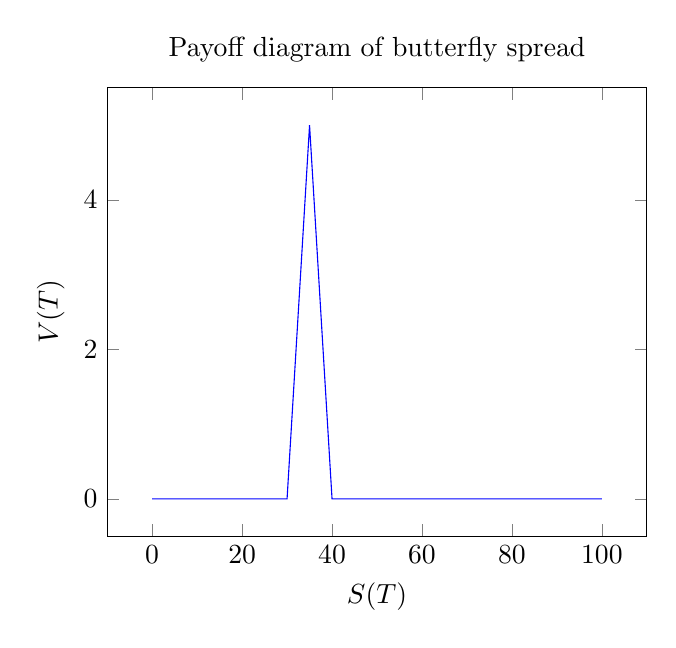
\begin{tikzpicture}[
    declare function={
        value(\x) = (\x <= 30) * (0) +
            and(\x > 30, \x <= 35) * (\x - 30) +
            and(\x > 35, \x <= 40) * (\x - 30 - 2 * (\x - 35)) +
            (\x > 40) * (\x - 30 - 2 * (\x - 35) + \x - 40);
    }
]
    \begin{axis}[
        title=Payoff diagram of butterfly spread,
        xlabel={$ S(T) $},
        ylabel={$ V(T) $},
    ]
        \addplot [
            blue,
            domain=0:100,
            samples=101,
        ]
            {value(x)};
    \end{axis}
\end{tikzpicture}

\subsection{Question 12}
Draw the payoff diagram at maturity of a bull spread with a long position in a
    call with strike 30 and short a call with strike 35, and of a bear spread
    with long a put of strike 20 and short a put of strike 15.

\paragraph{Answer}
Payoffs of the call options in bull spread at maturity are:
\begin{align*}
    C_1(T) &= \max (S(T) - K_{C_1}, 0) = \max (S(T) - 30, 0); \\
    C_2(T) &= \max (S(T) - K_{C_2}, 0) = \max (S(T) - 35, 0). \\
\end{align*}
Payoffs of the put options in bear spread at maturity are:
\begin{align*}
    P_1(T) &= \max (K_{P_1} - S(T), 0) = \max (20 - S(T), 0); \\
    P_2(T) &= \max (K_{P_2} - S(T), 0) = \max (15 - S(T), 0). \\
\end{align*}
Value of the portfolios at maturity are
\begin{align*}
    V_{bull}(T) &= C_1(T) - C_2(T); \\
    V_{bear}(T) &= P_1(T) - P_2(T). \\
\end{align*}

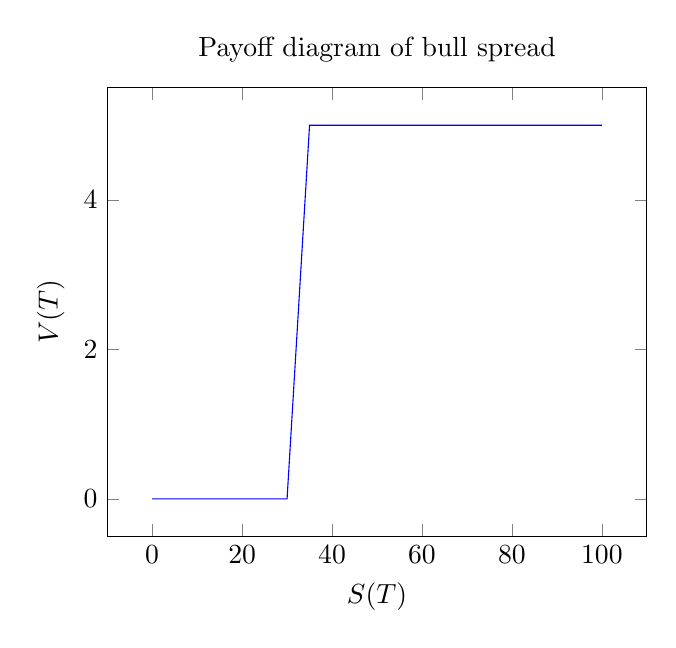
\begin{tikzpicture}[
    declare function={
        value(\x) = (\x <= 30) * (0) +
            and(\x > 30, \x <= 35) * (\x - 30) +
            (\x > 35) * (\x - 30 - (\x - 35));
    }
]
    \begin{axis}[
        title=Payoff diagram of bull spread,
        xlabel={$ S(T) $},
        ylabel={$ V(T) $},
    ]
        \addplot [
            blue,
            domain=0:100,
            samples=101,
        ]
            {value(x)};
    \end{axis}
\end{tikzpicture}%
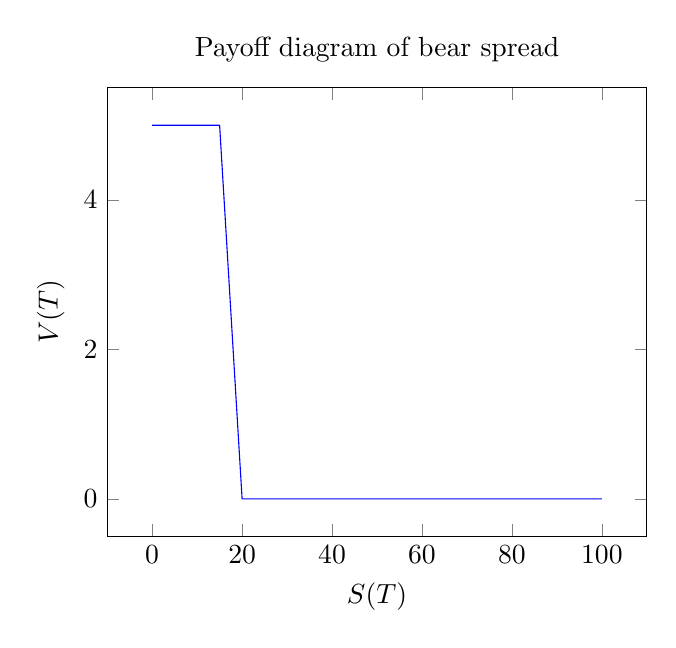
\begin{tikzpicture}[
    declare function={
        value(\x) = (\x <= 15) * (20 - \x - (15 - \x)) +
            and(\x > 15, \x <= 20) * (20 - \x) +
            (\x > 20) * (0);
    }
]
    \begin{axis}[
        title=Payoff diagram of bear spread,
        xlabel={$ S(T) $},
        ylabel={$ V(T) $},
    ]
        \addplot [
            blue,
            domain=0:100,
            samples=101,
        ]
            {value(x)};
    \end{axis}
\end{tikzpicture}

\subsection{Question 13}
Which of the following two portfolios would you rather hold:
\begin{itemize}
    \item Portfolio 1: Long one call option with strike $ K = X - 5 $ and long
        one call option with strike $ K = X + 5 $;
    \item Portfolio 2: Long two call options with strike $ K = X $?
\end{itemize}
(All options are on the same asset and have the same maturity.)

\paragraph{Answer}
Payoffs of the call options in Portfolio 1 at maturity are:
\begin{align*}
    C_1(T) &= \max (S(T) - (X - 5), 0); \\
    C_2(T) &= \max (S(T) - (X + 5), 0). \\
\end{align*}
Payoffs of the call options in Portfolio 2 at maturity are:
\begin{align*}
    C_3(T) &= \max (S(T) - X, 0). \\
\end{align*}
Value of the portfolios at maturity are
\begin{align*}
    V_1(T) &= C_1(T) + C_2(T) = \max (S(T) - (X - 5), 0) +
        \max (S(T) - (X + 5), 0); \\
    V_2(T) &= 2 C_3(T) = 2 \max (S(T) - X, 0).
\end{align*}

Long Portfolio 1 and short Portfolio 2 is equivalent to long a butterfly
    spread, which is always non-negative at maturity.
Therefore, it is better owning Portfolio 1 since its payoff at maturity will
    always be at least as big as the payoff of Portfolio 2.

\subsection{Question 14}
Call options with strikes 100, 120, and 130 on the same underlying asset and
    with the same maturity are trading for 8, 5, and 3, respectively (there is
    no bid-ask spread).
Is there an arbitrage opportunity present?
If yes, how can you make a riskless profit?

\paragraph{Answer}
For arbitrage opportunity to be present, the portfolio must have non-negative
    payoff at maturity and with a negative cost setting up.

Let $ K_1 = 100 < K_2 = 120 < K_3 = 130 $ be the strike of the options.
Let $ x_1 $, $ x_2 $, and $ x_3 $ be options positions at time 0.
The portfolio value at time 0 is
\begin{equation*}
    V(0) = x_1 C_1(0) + x_2 C_2(0) + x_3 C_3(0).
\end{equation*}
The portfolio value at maturity $ T $ is
\begin{align*}
    V(T) &= x_1 C_1(T) + x_2 C_2(T) + x_3 C_3(T) \\
         &= x_1 \max (S(T) - K_1, 0) + x_2 \max (S(T) - K_2, 0) +
            x_3 \max(S(T) - K_3, 0)
\end{align*}
The payoff at maturity is as follows:
\begin{table}
    \begin{center}
        \begin{tabular}[c]{l|l}
            \hline
            \multicolumn{1}{c|}{\textbf{S(T)}} &
            \multicolumn{1}{c}{\textbf{V(T)}} \\
            \hline
            $ S(T) \leq K_1 $ & 0 \\
            $ K_1 < S(T) \leq K_2 $ & $ x_1 S(T) - x_1 K_1) $  \\
            $ K_2 < S(T) \leq K_3 $ & $ (x_1 + x_2) S(T) - x_1 K_1 -
                x_2 K_2 $ \\
            $ K_3 < S(T) $ & $ (x_1 + x_2 + x_3) S(T) - x_1 K_1 -
                x_2 K_2 - x_3 K_3 $\\
            \hline
        \end{tabular}
    \end{center}
\end{table}

$ V(T) $ is non-negative when $ S(T) \leq K_2 $ only if a long position is
    taken for the option with strike $ K_1 $, i.e., $ x_1 \geq 0 $.
$ V(T) $ is non-negative for any value of $ S(T) $ if and only if
    $ x_1 \geq 0 $, if $ V(T) $ when $ S(T) = K_3 $ is non-negative, and if
    $ x_1 + x_2 + x_3 \geq 0 $.

An arbitrage exists if and only if the values $ C_1(0) $, $ C_2(0) $,
    $ C_3(0) $ are such that the we find $ x_1 $, $ x_2 $, and $ x_3 $ with the
    following properties:
\begin{align*}
    x_1 C_1(0) + x_2 C_2(0) + x_3 C_3(0) &< 0; \\
    x_1 &\geq 0; \\
    (x_1 + x_2) K_3 - x_1 K_1 - x_2 K_2 &\geq 0; \\
    x_1 + x_2 + x_3 &\geq 0.
\end{align*}

For $ C_1(0) = 8 $, $ C_2(0) = 5 $, $ C_3(0) = 3 $ and $ K_1 = 100 $,
    $ K_2 = 120 $, $ K_3 = 130 $, the problem becomes finding $ x_1 \geq 0 $,
    $ x_2 $, and $ x_3 $ such that
\begin{align*}
    8 x_1 + 5 x_2 + 3 x_3 &< 0; \\
    30 x_1 + 10 x_2 &\geq 0; \\
    x_1 + x_2 + x_3 &\geq 0.
\end{align*}

Arbitrage can occur for a portfolio with long positions in the options with
    lowest and highest strikes and a short position in the option with the
    middle strike.
Choosing $ x_3 = -x_1 - x_2 $, the constraints become
\begin{align*}
    5 x_1 + 2 x_2 &< 0; \\
    3 x_1 + x_2 &\geq 0. \\
\end{align*}
The constraints are satisfied when
\begin{equation*}
    x_1 = 1; \quad x_2 = -3; \quad  x_3 = 2.
\end{equation*}

Buying one option with strike 100, selling three options with strike 120, and
    buying two options with strike 130 will generate a positive cash flow of
    \$1, and will result in a portfolio that will not lose money, regardless of
    the value of the underlying asset at maturity of the options.

\subsection{Question 15}
A stock with spot price 40 pays dividends continuously at a rate of 3\%.
The four months at-the-money put and call options on this asset are trading at
\$2 and \$4, respectively.
The risk-free rate is constant and equal to 5\% for all times.
Show that the Put-Call parity is not satisfied and explain you would take
    advantage of this arbitrage opportunity.

\paragraph{Answer}
Given the following values: $ S = 40 $, $ K = 40 $, $ q = 0.03 $, $ C = 4 $,
    $ P = 2 $, $ r = 0.05 $, $ T = 1 / 3 $, we have
\begin{equation*}
    P + S e^{-qT} - C = \approx 37.6020 < 39.3389 \approx K e^{-rT}
\end{equation*}
To take advantage of the arbitrage opportunity, we:
\begin{enumerate}
    \item Short one call (+ \$4)
    \item Long one put (- \$2)
    \item Short one forward-like position
        \begin{itemize}
            \item Short one share (- \$39.6020)
            \item Invest in risk-free bond (+ \$39.3389)
        \end{itemize}
\end{enumerate}
The riskless profit at maturity will be approximately \$1.74.

\subsection{Question 16}
The bid and ask prices for a six months European call option with strike 40 on
    a non-dividend-paying stock with spot price 42 are \$5 and \$5.5,
    respectively.
The bid and ask prices for a six months European put option with strike 40 on
    the same underlying asset are \$2.75 and \$3.25, respectively.
Assume that the risk free rate is equal to 0.
Is there an arbitrage opportunity present?

\paragraph{Answer}
The Put-Call parity is
\begin{align*}
    C - P &= S - K \\
    C - P &= 42 - 40 = 2
\end{align*}
An arbitrage opportunity exists if $ C - P $ can be ``bought" for less than \$2,
    of ``sold" for more than \$2.

The bid-ask spreads are
\begin{align*}
    C &\in [5, 5.5] \\
    P &\in [2.75, 3.25]
\end{align*}
Thus, the possible range of $ C - P $ is $ C - P \in [1.75, 2.75] $.

Since $ C - P $ can be ``bought" for more than \$2 and ``sold" for less than
    \$2, there is no arbitrage opportunity.

\subsection{Question 17}
You expect that an asset with spot price \$35 will trade in the \$40 - \$45
    range in one year.
One year at-the-money (ATM) calls on the asset can be bought for \$4.
To act on the expected stock price appreciation, you decide to either buy the
    asset, or to buy ATM calls.
Which strategy is better, depending on where the asset price will be in a year?

\paragraph{Answer}
Payoff for the strategy of buying the asset is
\begin{equation*}
    V_1(T) = \frac{x}{35} S(T),
\end{equation*}
where $ x $ is the amount invested and $ S(T) $ is the spot price of the asset
    in one year.

Payoff for the strategy of buying call option is
\begin{equation*}
    V_2(T) = \frac{x}{4} \max (S(T) - 35)
\end{equation*}

If the asset price is less than \$35 in a year, the calls will expire worthless
    while the first strategy of buying the asset will not lose all its value.
However, the strategy of buying call options can be more profitable if the
    asset appreciates in value, i.e., the spot price is larger than \$35.
The break even point of the two strategies is approximately \$39.5161, since
\begin{equation*}
    \frac{x}{35} S(T) = \frac{x}{4} \max (S(T) - 35) \Leftrightarrow
        S(T) = 39.5161
\end{equation*}
If the price of the asset is expected to be \$40 - \$45, buying call options
    will be the more profitable strategy.

\subsection{Question 18}
The risk free rate is 8\% compounded continuously and the dividend yield of a
    stock index is 3\%.
The index is 12,000 and the futures prices of a contract deliverable in three
    months is 12,100.
Is there an arbitrage opportunity, and how would you take advantage of it?

\paragraph{Answer}
Futures fair price is given by
\begin{align*}
    S e^{(r - q)T} &= 12000 e^{(0.08 - 0.03)/4} \\
                   &= 12150.94 \\
                   &> 12100
\end{align*}
The futures contract is underpriced.
To take advantage of the arbitrage opportunity, we long the future and short
    the index (spot).

At maturity, the asset is bought for 12100 and the short is closed.
The realized gain is the interest on the cash from the short position minus
    12,100, i.e.,
\begin{equation*}
    e^{0.08/4} (12000 e^{-0.03/4}) - 12100 = 50.94
\end{equation*}
